\section{Multivariate depth functions}

\begin{figure}
    \centering
    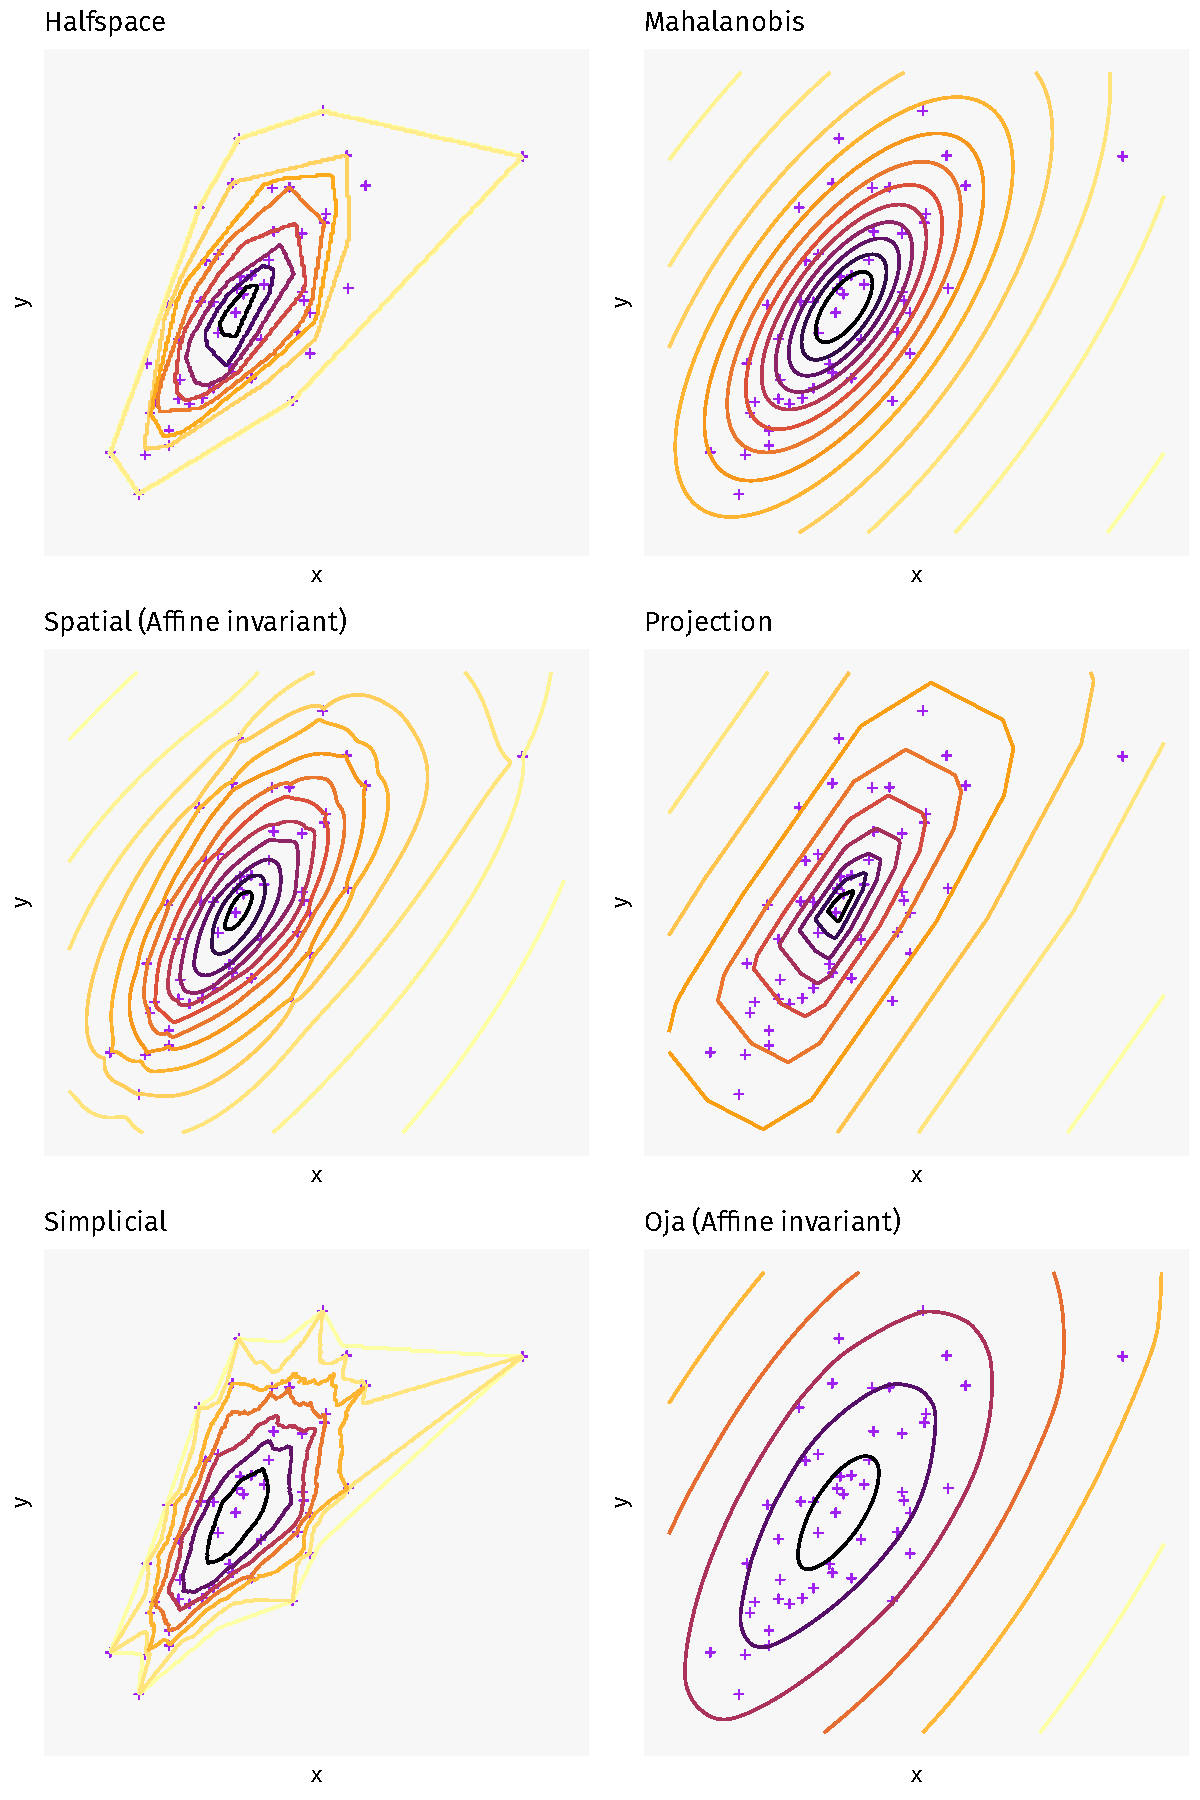
\includegraphics[width = \textwidth, page = 1]{contours}
    \caption{
        Depth contours with respect to purple points.
    }
    \label{fig:depthcontours}
\end{figure}


\begin{definition}[Halfspace/Tukey depth]
    Denote the collection of all closed halfspaces in $\R^d$ containing $\vx$
    by $\mathcal{H}_{\vx}$.
    The halfspace depth, or Tukey depth, is defined as
    \begin{equation}
        D_H(\vx, F) = \inf_{H \in \mathcal{H}_{\vx}} P_{F}(H).
    \end{equation}
\end{definition}

\begin{remark}
    If $F \in \mathscr{F}$ is supported on a convex region $C \subset \R^d$,
    then $D(\Cdot, F)$ vanishes outside $C$.
\end{remark}

\begin{proposition}
    The halfspace depth can be formulated as
    \begin{equation}
        D_H(\vx, F) = \inf_{\vv \in S^{d - 1}} P_{\vX \sim F}(\ip{\vv}{\vX} \leq \ip{\vv}{\vx}).
    \end{equation}
\end{proposition}

\begin{remark}
    When $d = 1$, the halfspace depth reduces to
    \begin{equation}
        D_H(x, F) = \min\{P_F(-\infty, x],\, P_F[x, \infty)\}.
    \end{equation}
\end{remark}

% \textcite{albertos-reyes-2008b} showed that the halfspace depth fully
% characterizes discrete measures with countable support.
% This is a generalization of a result by \textcite{koshevoy-2002}.

% \begin{theorem}[\cite{albertos-reyes-2008b}]
%     Let $F_1, F_2 \in \mathscr{F}$ where $F_1$ is a discrete measure with
%     countable support.
%     If $D_H(\vx, F_1) = D_H(\vx, F_2)$ for all $\vx \in \R^d$ then $F_1 =
%     F_2$.
% \end{theorem}

\textcite{struyf-rousseeuw-1999} showed that halfspace depth fully
characterizes empirical distributions.

\begin{theorem}[\cite{struyf-rousseeuw-1999}]
    The empirical distribution of any dataset $\{\vX_i\}_{i = 1}^n \subset
    \R^d$ is uniquely determined by its halfspace depth function $D(\Cdot,
    \hat{F}_n)$.
\end{theorem}

\textcite{nagy-2020} offers a comprehensive overview of this characterization
problem.
Indeed, \textcite{nagy-2021} supplies examples of distinct probability
distributions $F_1, F_2$ such that $D_H(\Cdot, F_1) = D_H(\Cdot, F_2)$.
It can be shown that for an $\alpha$-symmetric distribution $F$ that $D_H(\vx,
F) = G(-\norm{\vx}_{\alpha^*})$, where $G$ is the marginal distribution of the
first component of $\vX \sim F$ and $1/\alpha + 1/\alpha^* = 1$.



\begin{definition}[Mahalanobis depth]
    Let $\vX \sim F$ have mean $\vmu$ and covariance matrix $\Sigma$.
    The Mahalanobis depth is defined as
    \begin{equation}
        D_{M}(\vx, F) = \left(1 + (\vx - \vmu)^\top \Sigma^{-1}(\vx - \vmu)\right)^{-1}.
    \end{equation}
\end{definition}

\begin{remark}
    The mean and covariance in the above definition may be replaced with more
    robust estimates $\vmu^*$ and $\Sigma^*$, for instance using the minimum
    covariance determinant (MCD) method.
    The corresponding depth function is called the robust Mahalanobis depth.
\end{remark}

\begin{definition}[Spatial depth]
    The spatial depth is defined as
    \begin{equation}
        D_{Sp}(\vx, F) = 1 - \left\Vert \E_{\vX \sim F}\left[\frac{\vx - \vX}{\norm{\vx - \vX}}\right] \right\Vert.
    \end{equation}
    We use the convention $\bm0/0 = \bm0$.
\end{definition}

\begin{remark}
    Spatial depth defined as above does not obey \textbf{P1}.
    Indeed, spatial depth is only invariant under spherical transformations of
    the form $U\vX + \bm{b}$ for orthonormal $U$.
    We may define an affine invariant version of spatial depth as
    \begin{equation}
        D_{AISp}(\vx, F) = 1 - \left\Vert \E_{\vX \sim F}\left[\frac{\Sigma^{-1/2}(\vx - \vX)}{\sqrt{(\vx - \vX)^\top\Sigma^{-1}(\vx - \vX)}}\right] \right\Vert.
    \end{equation}
\end{remark}

\begin{remark}
    \textcite{nagy-2017} showed that spatial depth does not obey \textbf{P3}.
\end{remark}

\begin{lemma}\label{lem:spatial_vanish}
    Spatial depth obeys \textbf{P4}, i.e.\ $D_{Sp}(\vx, F) \to 0$ as
    $\norm{\vx} \to \infty$.
\end{lemma}
\begin{proof}
    Let $\epsilon > 0$, and let $M > 0$ such that $P_{\vX \sim F}(\norm{\vX} >
    M) = \epsilon$.
    Denote $\vY = (\vx - \vX) / \norm{\vx - \vX}$, and observe that
    \begin{equation}
        \E_{\vX \sim F}\left[\vY\right]
        = (1 - \epsilon)\E\left[\vY\mid \norm{\vX} \leq M\right] +
          \epsilon\E\left[\vY\mid \norm{\vX} > M\right]
    \end{equation}
    Thus, using $\norm{\vY} = 1$ and the reverse triangle inequality,
    \begin{equation}
        \norm{\E\left[\vY\right]}
        \geq (1 - \epsilon)\norm{\E\left[\vY\mid \norm{\vX} \leq M\right]} - \epsilon.
    \end{equation}
    Let $\alpha = \arccos((1 - 2\epsilon)/(1 - \epsilon))$, and let $r_\alpha =
    M/\sin\alpha$.
    It follows that the ball $\{\vx \in \R^d\colon \norm{\vx} \leq M\}$
    subtends an angle of at most $2\alpha$ from any point $\vx$ such that
    $\norm{\vx} > r_\alpha$.
    This gives $\norm{\E[\vY \mid \norm{\vX} \leq M]} \geq \cos\alpha$.
    Thus, for $\norm{\vx} > r_\alpha$,
    \begin{equation}
        \norm{\E[\vY]} \geq (1 - \epsilon)\cos\alpha - \epsilon = 1 - 3\epsilon,
    \end{equation}
    whence $D_{Sp}(\vx, F) \leq 3\epsilon$.
\end{proof}



\begin{definition}[Projection depth]
    The projection depth is defined as
    \begin{equation}
        D_P(\vx, F) = \left(1 + \sup_{\vv \in S^{d - 1}} \frac{|\ip{\vv}{\vx} - \med(\ip{\vv}{\vX})|}{\MAD(\ip{\vv}{\vX})}\right)^{-1}, \quad
        \vX \sim F.
    \end{equation}
\end{definition}

\begin{definition}[Simplicial depth]
    The simplicial depth is defined as
    \begin{equation}
        D_{Sim}(\vx, F) = P_{\vX_i \iid F}(\vx \in \conv(\vX_1, \dots, \vX_{d + 1})),
    \end{equation}
    where $\conv(\vx_1, \dots, \vx_{d + 1})$ denotes the convex hull of $\{\vx_1, \dots, \vx_{d + 1}\}$.
\end{definition}

\begin{definition}[Oja depth]
    The simplicial volume depth, or Oja depth, is defined as
    \begin{equation}
        D_{Oja}(\vX, F) = \left(1 + \E_{\vX_i \iid F}\left[\vol(\conv(\vx, \vX_1, \dots, \vX_d))\right]\right)^{-1}.
    \end{equation}
\end{definition}

\begin{remark}
    Oja depth does not obey \textbf{P1}, since
    \begin{equation}
        \vol(\conv(A\vx_1 + \bm{b}, \dots, A\vx_{d + 1} + \bm{b})) = |\det(A)| \vol(\conv(\vx_1, \dots, \vx_{d + 1})).
    \end{equation}
    Instead, we may define an affine invariant version of Oja depth as
    \begin{equation}
        D_{AIOja}(\vX, F) = \left(1 + \E_{\vX_i \iid F}\left[\frac{\vol(\conv(\vx, \vX_1, \dots, \vX_d))}{\sqrt{\det(\Sigma)}}\right]\right)^{-1},
    \end{equation}
    where $\Sigma$ is the covariance matrix of $F$.
\end{remark}


\subsection{The projection property}


\begin{definition}[Projection property]
    We say that a depth function $D$ has the projection property if
    \begin{equation}
        D(\vx, F_{\vX}) = \inf_{\vv \in S^{d - 1}} D(\ip{\vv}{\vx}, F_{\ip{\vv}{\vX}}).
    \end{equation}
\end{definition}

Depths which have this property can be approximated by calculating the
univariate depths of the projected data along many directions $\vv$.

\begin{lemma}
    The halfspace depth, Mahalanobis depth, and projection depth have the
    projection property.
\end{lemma}

The halfspace depth in particular is often computationally challenging.
Thus, the property motivates the definition of the random Tukey depth
\parencite{albertos-reyes-2008a}.

\begin{definition}[Random Tukey depth]
    Let $\vv_1, \dots, \vv_n$ be a realization of an iid sample from $\UU(S^{d
    - 1})$.
    The random Tukey depth is defined as
    \begin{equation}
        D_{RT}(\vx, F_{\vX}) = \min_{1 \leq i \leq n} D_H(\ip{\vv_i}{\vx}, F_{\ip{\vv_i}{\vX}}).
    \end{equation}
\end{definition}



\subsection{Continuity properties}

It is also desirable for a depth function to obey some notions of continuity.
\begin{enumerate}
    \item[\textbf{C1}.] \emph{Continuity in $\vx$.}
    \begin{equation}
        D(\vx_n, F) \to D(\vx, F)\;\text{ when }\; \vx_n \to \vx.
    \end{equation}

    \item[\textbf{C2}.] \emph{Continuity in $F$.}
    \begin{equation}
        D(\vx, F_n) \to D(\vx, F)\;\text{ when }\; F_n \tod F.
    \end{equation}

    \item[\textbf{C3}.] \emph{Uniform continuity}.
    \begin{equation}
        \sup_{\vx \in G} |D(\vx, F_n) - D(\vx, F)| \to 0\;\text{ when }\; F_n \tod F.
    \end{equation}
\end{enumerate}

Property \textbf{C1} is rarely satisfied without imposing some regularity
conditions on $F$, such as absolute continuity.
Property \textbf{C2} helps bridge the gap between the population and empirical
versions of depth.
Property \textbf{C3} becomes relevant when dealing with the convergence of
depth contours.


The Mahalanobis depth is trivially continuous in $\vx$, i.e.\ obeys
\textbf{C1}.
Furthermore, it also satisfies \textbf{C2} as long as $F$ has a regular
covariance matrix \parencite{mosler-mozharovskyi-2022}.


The halfspace depth also enjoys all three notions of continuity, under mild
restrictions on $F$.

\begin{theorem}[\cite{mizera-volauf-2002}]
    Let $F \in \mathscr{F}$ be such that the probability of every hyperplane
    in $\R^d$ is zero, i.e.\ for all $\alpha \in \R$ and $\vv \in S^{d - 1}$,
    \begin{equation}
        P_{\vX \sim F}(\ip{\vv}{\vX} = \alpha) \;=\; 0. \label{eq:halfspace_continuity}
    \end{equation}
    Then for $\vx_n \to \vx$ and $F_n \tod F$, we have $D_H(\vx_n, F_n) \to
    D_H(\vx, F)$.
\end{theorem}
\begin{remark}
    Equation~\ref{eq:halfspace_continuity} is satisfied whenever $F$ is
    absolutely continuous.
\end{remark}
\begin{remark}
    It follows that if $F \in \mathscr{F}$ satisfies
    Equation~\ref{eq:halfspace_continuity}, then the map $D_H(\Cdot, F)$ is
    continuous.
\end{remark}

\begin{corollary}
    Let $F \in \mathscr{F}$ satisfy Equation~\ref{eq:halfspace_continuity}.
    Then, for $F_n \tod F$, and compact $K \subset \R^d$,
    \begin{equation}
        \sup_{\vx \in K} |D_H(\vx, F_n) - D_H(\vx, F)| \to 0.
    \end{equation}
\end{corollary}
\begin{proof}
    Denoting $g = D(\Cdot, F)$, $g_n = D_H(\Cdot, F_n)$, we have the
    continuity of $g$ along with $g_n(\vx_n) \to g(\vx)$ whenever $\vx_n \to
    \vx$ in $K$.
    If the given conclusion is false, we may pass to a subsequence of $g_n$
    and find $\epsilon > 0$ such that each $\sup_{\vx \in K} |g_n(\vx) -
    g(\vx)| \geq \epsilon$.
    Using the compactness of $K$, we pass to a further subsequence and find
    $\vx \in K$ such that $\vx_n \to \vx$.
    This contradicts $|g_n(\vx_n) - g(\vx_n)| \geq \epsilon$.
\end{proof}

\begin{theorem}\label{thm:halfspace_uniform}
    Let $F \in \mathscr{F}$ satisfy Equation~\ref{eq:halfspace_continuity}.
    Then, for $F_n \tod F$,
    \begin{equation}
        \sup_{\vx \in \R^d} |D_H(\vx, F_n) - D_H(\vx, F)| \to 0.
    \end{equation}
\end{theorem}
\begin{proof}
    Let $K_r = \{\vx \in \R^d\colon \norm{\vx} \leq r\}$ be a continuity set
    of $F$.
    Observe that $D_H(\vy, F) \leq P_F(K_r^c)$ for $\vy \in K_r^c$, hence
    \begin{equation}
        \sup_{\vy \in K_r^c} |D_H(\vy, F_n) - D_H(\vy, F)| \leq P_{F_n}(K_r^c) + P_F(K_r^c).
    \end{equation}
    As $n \to \infty$, we have $P_{F_n}(K_r^c) \to P_F(K_r^c) = p_r$ (say).
    Thus, denoting $\delta_n(X) = \sup_{\vx \in X} |D_H(\vx, F_n) - D_H(\vx,
    F)|$, we have
    \begin{align}
        \limsup_{n \to \infty} \delta_n(\R^d)
        &\leq \lim_{n \to \infty} \delta_n(K_r) + \limsup_{n \to \infty} \delta_n(K_r^c) \\
        &\leq 0 + 2p_r.
    \end{align}
    Using $p_r \to 0$ as $r \to \infty$ completes the proof.
\end{proof}



The spatial depth is similarly well behaved.

\begin{theorem}
    Spatial depth obeys \textbf{C1} when $F$ is non-atomic, as well as
    \textbf{C2}.
\end{theorem}
\begin{proof}
    Consider the spatial map
    \begin{equation}
        S_F\colon \R^d \to \R^d, \qquad
        \vx \mapsto \E_{\vX \sim F}\left[\frac{\vx - \vX}{\norm{\vx - \vX}}\right].
    \end{equation}
    The Dominated Convergence Theorem guarantees the continuity of $S_F$,
    hence of $D_{Sp}(\Cdot, F) = 1 - \norm{S_F(\Cdot)}$.
    Furthermore, if $F_n \tod F$, we have $S_{F_n}(\vx) \to S_F(\vx)$ by the
    Portmanteau Lemma for all $\vx \in \R^d$.
\end{proof}

\begin{theorem}[\cite{serfling-2002}]
    For $F \in \mathscr{F}$ and compact $K \subset \R^d$,
    \begin{equation}
        \sup_{\vx \in K} |D_{Sp}(\vx, \hat{F}_n) - D_{Sp}(\vx, F)| \toas 0.
    \end{equation}
\end{theorem}

\begin{remark}
    This result can be generalized from compact subsets $K$ to the whole of
    $\R^d$, using Lemma~\ref{lem:spatial_vanish} and arguments similar to the
    proof of Theorem~\ref{thm:halfspace_uniform}.
\end{remark}


